\documentclass{article}
\usepackage{array}
\usepackage[column=0]{cellspace}
\setlength\cellspacetoplimit{6pt}
\setlength\cellspacebottomlimit{6pt}
\usepackage{graphicx} % Required for inserting images
\usepackage{amsmath}
\usepackage{amssymb}
\usepackage{amsthm}
\usepackage{amsfonts}
\usepackage{gensymb}
\newcommand{\myvec}[1]{\ensuremath{\begin{pmatrix}#1\end{pmatrix}}}

\title{MathConstruction}

\begin{document}

\section{NCERT 12.10.5.9}

Find the position vector of a point R which divides the line joining two points P and Q whose Position Vectors are $2\vec{a}+\vec{b}$ and $\vec{a}-3\vec{b}$ externally in the ration $1:2$.Also, Show that P is the mid point of the line segment RQ \\
\textbf{Construction steps:}
\begin{enumerate}

    \item Let us, Consider Position vectors 
    \begin{table}[!ht]
        \centering
        \label{tab:3x3-margins}
        \begin{tabular}{|0c|0c|0c|}
            \hline
            \textbf{Symbol} & \textbf{value} & \textbf{Description} \\
            \hline
            P & $\myvec{x_1\\y_1}$ & position vector P \\
            \cline{1-1} \cline{2-2} \cline{3-3}
            Q & $\myvec{x_2\\y_2}$ & position vector Q \\
            \cline{1-1} \cline{2-2} \cline{3-3}
            \hline
        \end{tabular}
    \end{table}
    and the ratio is 
    \begin{align}
        m:n
    \end{align}
    For finding the position vector R,
    \begin{align}
        R=\frac{n(x_1,y_1)-m(x_2,y_2)}{n-m}
    \end{align}
    \item Now The position vectors P,Q and R are
    \begin{table}[!ht]
        \centering
        \label{tab:3x3-margins}
        \begin{tabular}{|0c|0c|0c|}
            \hline
            \textbf{symbol} & \textbf{Value} & \textbf{Description} \\
            \hline
            R & $\myvec{\frac{n.x_1-m.x_2}{n-m}\\ \frac{n.y_1-m.y_2}{n-m}}$ & position vector P \\
            \hline
        \end{tabular}
    \end{table}
    For showing P is the midpoint of the line segment RQ
    \begin{align}
        P=\frac{R+Q}{2}\\
        P=\myvec{x_1\\y_1}
    \end{align}
    So,it is proved that P is the midpoint of RQ.
    \item The Plot showing the Vector representation of the position vectors P,Q and R is
    \begin{figure}[!ht]
        \centering
        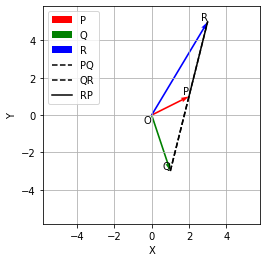
\includegraphics[width=\columnwidth]{/sdcard/geometry/math_computing/mathconstruction.png}
        \caption{point vectors P,Q,R}
        \label{fig:enter-label}
    \end{figure}
\end{enumerate}
\end{document}
